%!TEX root = minta_dolgozat.tex
%%%%%%%%%%%%%%%%%%%%%%%%%%%%%%%%%%%%%%%%%%%%%%%%%%%%%%%%%%%%%%%%%%%%%%%
\chapter{Forgalmi táblák}\label{ch:SIGNS}
%%%%%%%%%%%%%%%%%%%%%%%%%%%%%%%%%%%%%%%%%%%%%%%%%%%%%%%%%%%%%%%%%%%%%%%

\section{Mik a forgalmi táblák?}\label{sec:SIGNS:whatAreThey}

A forgalmi táblák a forgalom irányításáért felelősek; figyelmeztetik, irányítják és informálják a gépkocsivezetőket. Három fő típusú forgalmi tábla van és mindegyiknek különböző formával rendelkezik:
\begin{enumerate}
	\item utasító táblák (kör)
	\item figyelmeztető táblák (háromszög)
	\item informáló táblák (téglalap)
\end{enumerate}

Ez alól kivétel a "stop" tábla, ami nyolcszög alakú.

További információval szolgál a forgalmi tábláról a színe. A forgalmi táblák figyelemfelkeltőek kell legyenek, ennek megfelelően alkalmazzák a színeket is. A megjelenő színek: piros, fehér, fekete, sárga és kék. \citep{8}

A forgalmi táblák többsége két részből tevődik össze: egy külső telített sáv és egy belső szimbólum vagy szám. A belső szimbólum általában fekete. 


\section{Adathalmaz}\label{sec:SIGNS:dataSet}

Az adathalmazhoz egy forgalmi táblák felismerésére kitűzött németországi verseny adatait használtam fel.

\subsection{Tanulási adatok}

Az adathalmaz 1213 tanulási adatot tartalmaz. A képek mérete 16x16 pixeltől 128x128 pixelig változik, különböző szemszögből és változatos fényhatások mellett. A képek 43 kategóriába vannak sorolva, a tartalmazott forgalmi tábla alapján.

Habár nagy mennyiségű tanulási adat áll rendelkezésre, ezek nincsenek egyenlően elosztva az osztályok között. Ez megnehezíti a tanulást a neurális háló számára. Azok az osztályok amelyekben kevés tanulási adat van, kevésbé vannak befolyással a neurális háló kimenetére. 

\begin{figure}
\centering

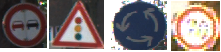
\includegraphics{images/train}
\caption{Példa tanulási adatokra}

\label{fig:trainingImage}
\end{figure}

A \ref{fig:trainingImage} ábrán látható példa négy tanítási adatra. Az első három képen levő táblák könnyedén felismerhetőek, míg a az utolsó tábla nehezen azonosítható. Nehéz megmondani, hogy 30-as, de 70-es vagy 80-as sebességkorlát. Az adathalmazban kis számban ugyan, de előfordulnak ehhez hasonló táblák. Ezek megnehezítik a tanulási folyamatot.

\subsection{Tesztelési adatok}

900 teszt adat állt a rendelkezésemre, amiken nullától hatig akárhány forgalmi tábla megjelenhetett. Ezek jóval nagyobb méretű képek a tanításra szánt képeknél, 1360x800 pixel nagyságúak. A \ref{fig:testImage} ábrán látható egy példa ilyen képre. Ezen a képen két forgalmi tábla található.

\begin{figure}[h]
\centering

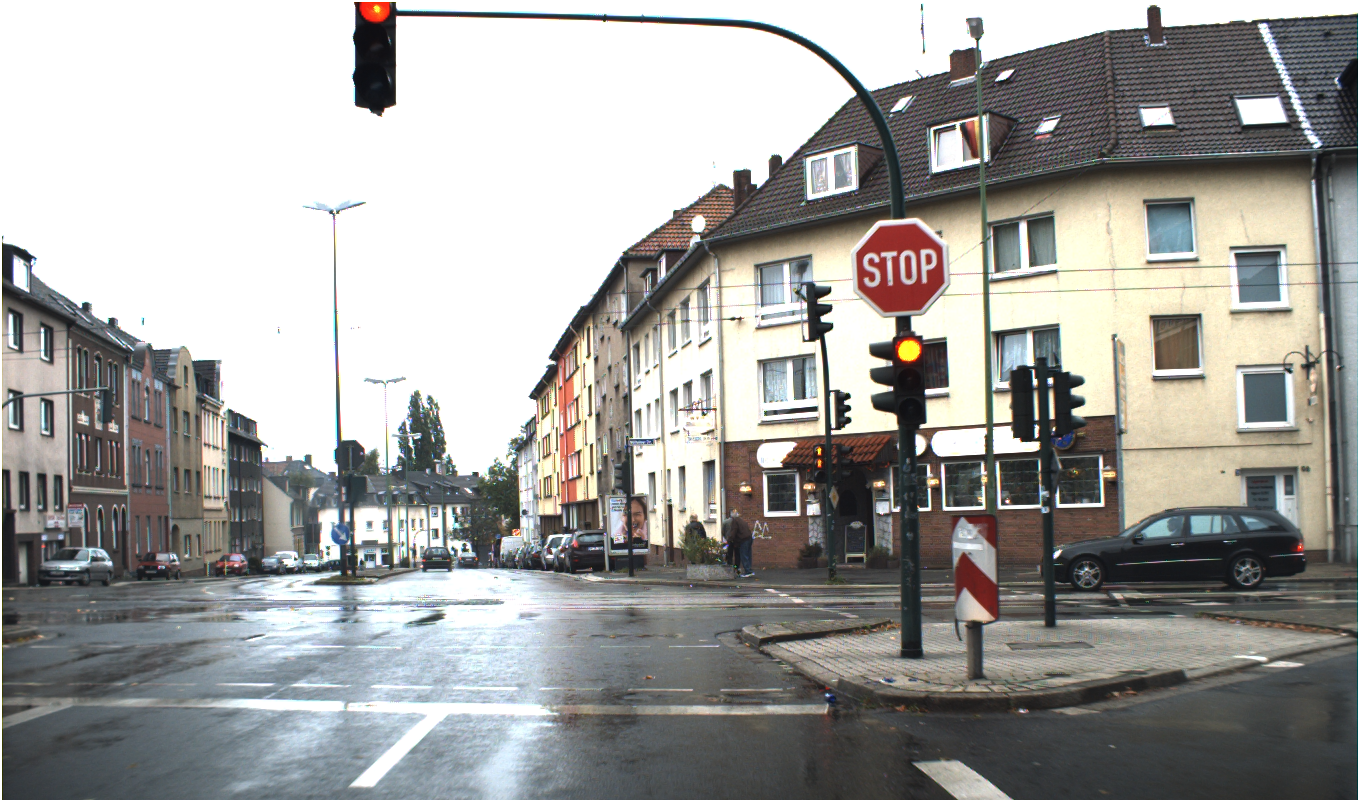
\includegraphics[scale=0.4]{testImage}
\caption{Példa teszt adatra}

\label{fig:testImage}
\end{figure}

